\ylDisplay{Peegel} % Ülesande nimi
{Tundmatu autor} % Autor
{piirkonnavoor} % Voor
{2012} % Aasta
{P 1} % Ülesande nr.
{1} % Raskustase
{
% Teema: Valgusõpetus
\ifStatement
Suure ruumi seinal on $2,0 m$ laiune peegel. Peegli kõrval, $0,5 m$ kaugusel peeglist ja $1,0 m$ kaugusel seinast, seisab inimene. Mööda peegli keskjoont tuleb peegli poole tema tuttav. Kui kaugel peeglist on peeglile lähenev inimene, kui tuttavad märkavad teineteist peeglis?
\begin{center}
	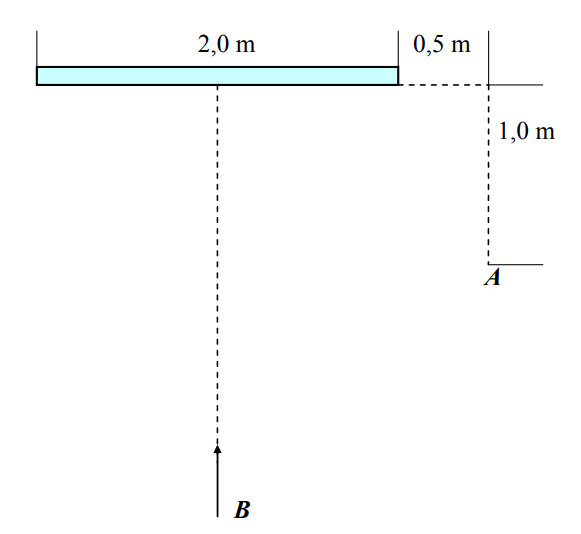
\includegraphics[width=0.5\linewidth]{2012-v2p-01-yl.PNG}
\end{center}
\fi


\ifHint
Kõige kaugemal on inimene peeglist siis, kui tema peegeldust on näha peegli nurgast. Ülesanne lahendub siis sarnaste kolmnurkade kaudu.
\fi

\ifSolution
\begin{center}
	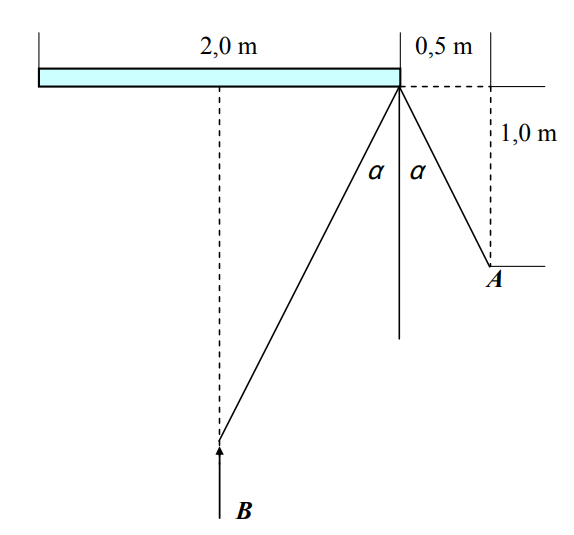
\includegraphics[width=0.5\linewidth]{2012-v2p-01-lah.PNG}
\end{center}
\fi
}
